% vim: ft=tex
\chapter{Requirements}\label{ch:reqs}
The requirements gathered during the first and second meeting with the client are
explained in this chapter. These are more concrete than the ones listed in the
Task Description in \autoref{ch:task-desc}.

First of all, these are the client's priorities:

\begin{enumerate}
\item Federation functionality, namely:
	\begin{enumerate}
		\item Topology definition
		\item DIM replication
		\item Message routing
	\end{enumerate}
\item \Gls{HA}
\item Persistence replication
\item Encryption (optional)
\item DIM access control
\item OPC UA \gls{HA} (optional)
\end{enumerate}

The following sections explain the requirements in greater detail, starting
with the functional ones. The non-functional requirements are described in
\autoref{sec:nfr}.

The functional requirements are each described in prosa as understood by the
students first and then formally in \gls{gherkin} style features. Those feature
specifications will later be useful to deduce test cases.

\section{Federation}
% TODO: big picture
Roadster will need to be run on multiple nodes in a hierarchical topology,
forming a distributed computing architecture. The root node would then act as
the client-facing server. This is formally specified in
\autoref{lst:feature:federation}. Typical node topologies include:

\begin{description}
	\item [ Single level with a single node ] \hfill\\
		This is the legacy setup and is what Roadster is already able
		to do. It consists of a single node. This is illustrated in
		\autoref{fig:topo:sl:noha}, where the single node is denoted as node R.

	\item [ Multi level ] \hfill\\
		This is the most basic federation setup. There is a root node, and
		a number of subnodes. Each subnode is directly connected to a number of field devices such as
		\glspl{PLC} or emergency phones. This is illustrated in
		\autoref{fig:topo:ml:noha}, where the root node is denoted as R
		and the subnodes as S1, S2, and S3.
\end{description}

\begin{figure}[]
	\center
	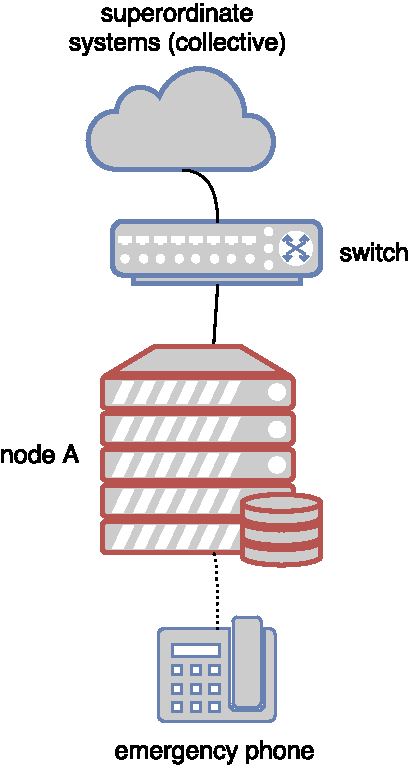
\includegraphics[width=0.2\textwidth]{img/topo_sl_noha.pdf}
	\source{mindclue GmbH}
	\caption{Logical federation topology example: Single level with a single node (legacy)}
	\label{fig:topo:sl:noha}
\end{figure}
\begin{figure}[]
	\center
	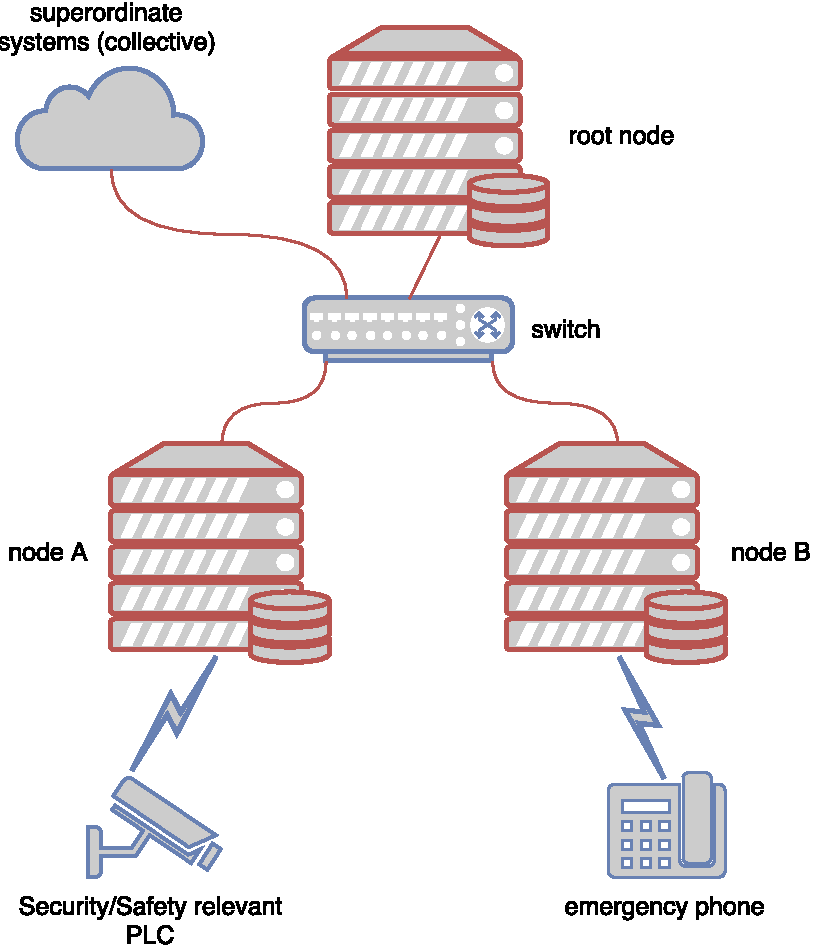
\includegraphics[width=0.6\textwidth]{img/topo_ml_noha.pdf}
	\source{mindclue GmbH}
	\caption{Logical federation topology example: Multi level}
	\label{fig:topo:ml:noha}
\end{figure}

% TODO: features are not listings
\begin{listing}
	\inputminted{Gherkin}{listings/features/federation/federation.feature}
	\caption{Formal feature: Federation}
	\label{lst:feature:federation}
\end{listing}

\paragraph{Network infrastructure} Roadster nodes would typically be connected
through a network switch, possibly assigned their own \gls{VLAN}. The root node
would typically have two \glspl{NIC}: One connected to the processing network,
i.e. the Roadster federation, and another one connected to the client network.

\subsection{DIM extension}

\subsubsection{Replication}
Extending the \gls{CSP} to keep the \gls{DIM} consistent across all nodes is a central
part of the federation functionality. This demands a replication of all modifications to
the dynamic subset of DIM objects to all other nodes in the federation.

\paragraph{Bidirection} Just like the CSP, bidirectional replication is required.
Because every node is authorative for its subset of objects in the
DIM, every node has to replicate modifications that have happened in the
meantime to its direct peers nodes, no matter if these peer nodes are
supernodes or subnodes.

According to the meta model in \autoref{fig:roadster:meta-model}, these dynamic
objects are exactly the instances of one of the following three
classes (marked yellow in the class diagram):
\begin{itemize}
	\item \rb{Roadster::Domain::Model::DataItem}
	\item \rb{Roadster::Domain::Model::Session}
	\item \rb{Roadster::Domain::Model::Case}
\end{itemize}

As described earlier, instances of these entity classes are marked "dirty" when
modified until they are replicated.

\subsubsection{Access control}
The aforementioned requirements imply that modifications to the \gls{DIM} can only be done by the
owning node. A node
must not modify objects owned by other nodes directly. This is to ensure that each node is its own source of truth
% FIXME: source of truth == ?
to all other nodes in the federation. Only the owner node can enforce a single
sequence of updates to its part of the DIM, which is necessary to guarantee
eventual consistency \cite[Chapter 5, Reliable Pub-Sub (Clone Pattern), Republishing
Updates from Clients]{zmq:zguide} across all actors of all nodes.

These two aspects to the DIM extension are formally specified in \autoref{lst:feature:federation:dimsync}

\begin{listing}
	\inputminted{Gherkin}{listings/features/federation/dim_extension.feature}
	\caption{Formal feature: DIM replication}
	\label{lst:feature:federation:dimsync}
\end{listing}

\subsection{Autonomy}
It is important that every node (and its subnodes) can keep up the operation autonomously even if the
link to its supernode fails or the supernode itself fails. This means that updates to
the \gls{DIM} must be possible even when neighboring nodes (including the supernode) are unavailable. After the
recovery from the outage, the \gls{DIM} replication shall be reinitiated so
all pending updates are shared to all other nodes as per normal operation.

This is formally specified in \autoref{lst:feature:federation:autonomy}.

\begin{listing}
	\inputminted{Gherkin}{listings/features/federation/autonomy.feature}
	\caption{Formal feature: Autonomy}
	\label{lst:feature:federation:autonomy}
\end{listing}

\subsection{Message routing}
There needs to be a message routing mechanism so a user
of one node's web UI can send a command (passed as a message) to another node where it will be
executed. An example for this is a forced value in the DIM to ignore the
actually measured value reported by a device in case the device is known to be
wrong. The common case where the command is issued at a higher level in the node
topology is priority. E.g. in a multi level setup with a root node R and two
subnodes S1 and S2, issuing a command on S1 for S2 has a low priority.

This is formally specified in \autoref{lst:feature:federation:cmdrouting}.

\begin{listing}
	\inputminted{Gherkin}{listings/features/federation/message_routing.feature}
	\caption{Formal feature: Message routing}
	\label{lst:feature:federation:cmdrouting}
\end{listing}

\section{High availability}
Roadster must be able to run in certain high availability setups. Achieving
this is done by adding redundant Roadster nodes.

The following additional federation topologies must be supported:
\begin{description}
	\item [ Single level \gls{HA} ] \hfill\\
		This is when there are exactly two nodes, both of them
		connected to the same set of field devices. The difference to a
		non-redundant case is the added backup node, forming a HA
		cluster. The field devices are thus connected to the HA cluster
		using two redundant paths. Both HA peers are able to interact
		with the field devices to perform operation tasks (e.g. reading
		sensor data, writing down configurations), but only one of them
		(the active one) must do so. This is illustrated in
		\autoref{fig:topo:sl:ha}.

	\item [ Multi level, \gls{HA} at root only ] \hfill\\
		There can be multiple hierarchy levels within a Roadster federation, such as two or
		three (anything else is declared out of scope of this thesis). Introducing
		redundancy is done at the root level in the form of a HA
		cluster, consisting of a primary and a backup node. An example of this setup is illustrated in
		\autoref{fig:topo:ml:ha}.
\end{description}

\begin{figure}[]
	\center
	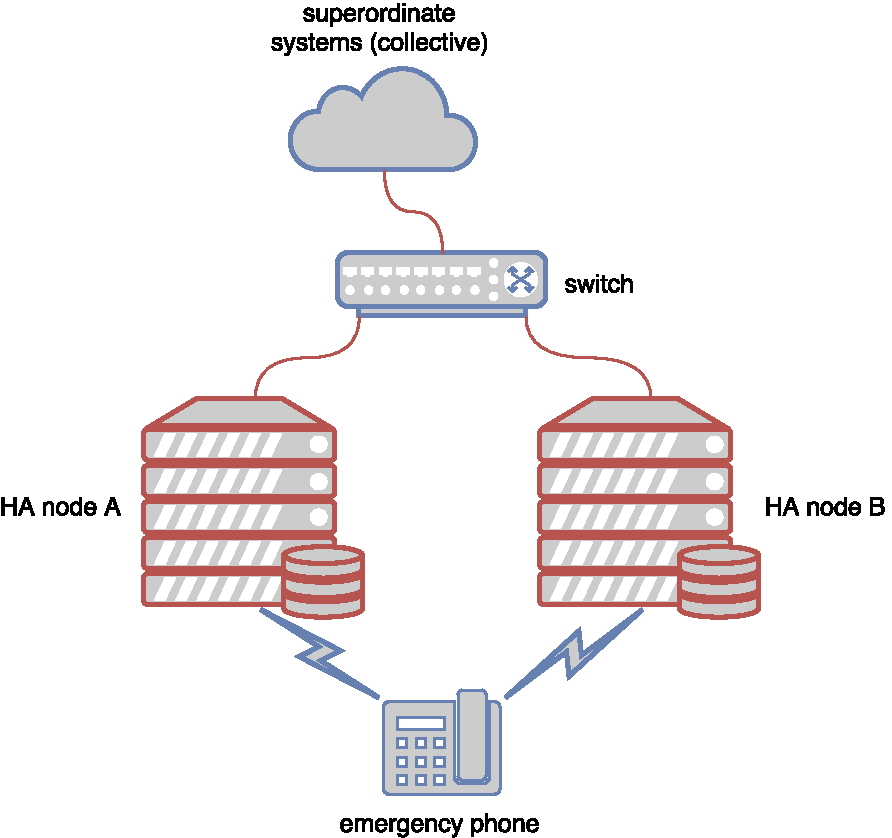
\includegraphics[width=0.5\textwidth]{img/topo_sl_ha.pdf}
	\caption{Federation example: a HA cluster and redundantly connected field devices}
	\label{fig:topo:sl:ha}
\end{figure}
\begin{figure}[]
	\center
	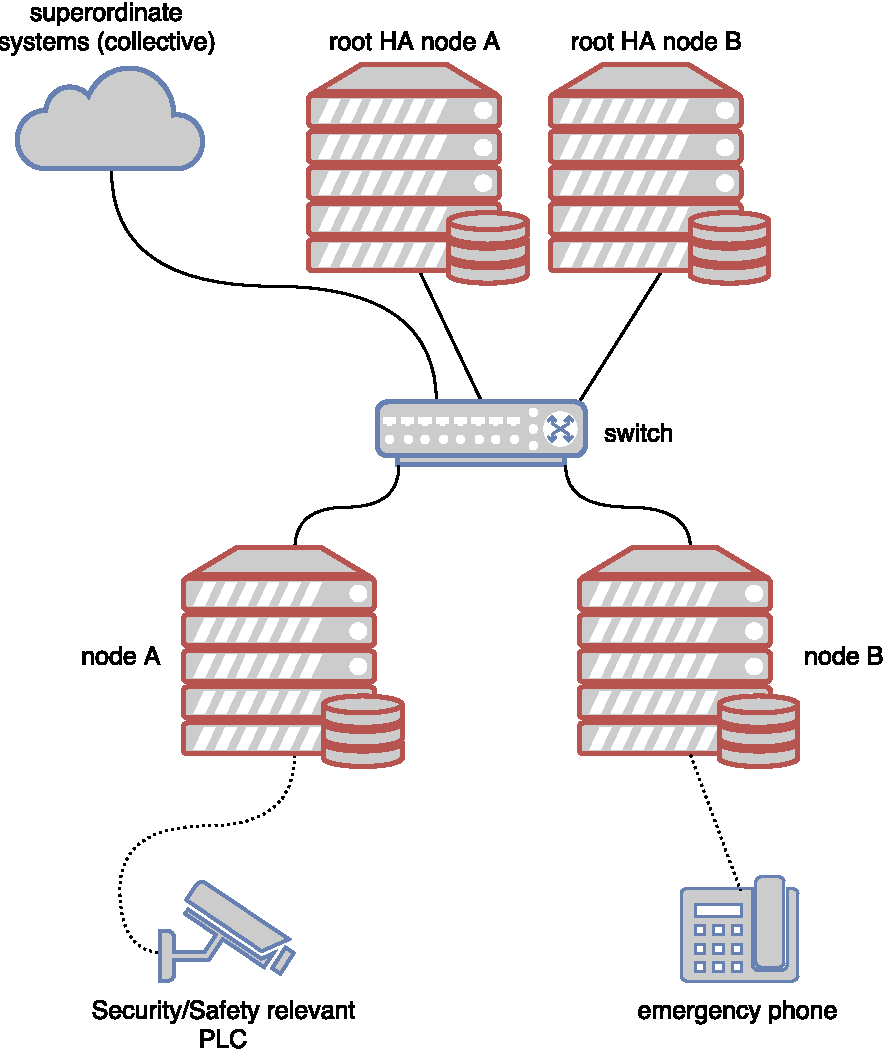
\includegraphics[width=0.5\textwidth]{img/topo_ml_ha.pdf}
	\caption{Federation example: HA cluster at root, two subnodes, each with field devices}
	\label{fig:topo:ml:ha}
\end{figure}

The following topologies are unusual, not planned for, and are thus declared
outside the scope of this thesis; however, they should be kept in mind so a
future extension to support them is feasible:

\begin{description}
	\item [ Multi level, \gls{HA} at bottom ] \hfill\\
	A single root node at the top and a subordinate HA pair each connected
	to the same field device.

	\item [ Multi level, \gls{HA} in the middle ] \hfill\\
	A single root node at the top, a subordinate HA pair, which in turn has
	a subordinate node connected to some field device.
\end{description}

\begin{figure}[]
	\center
	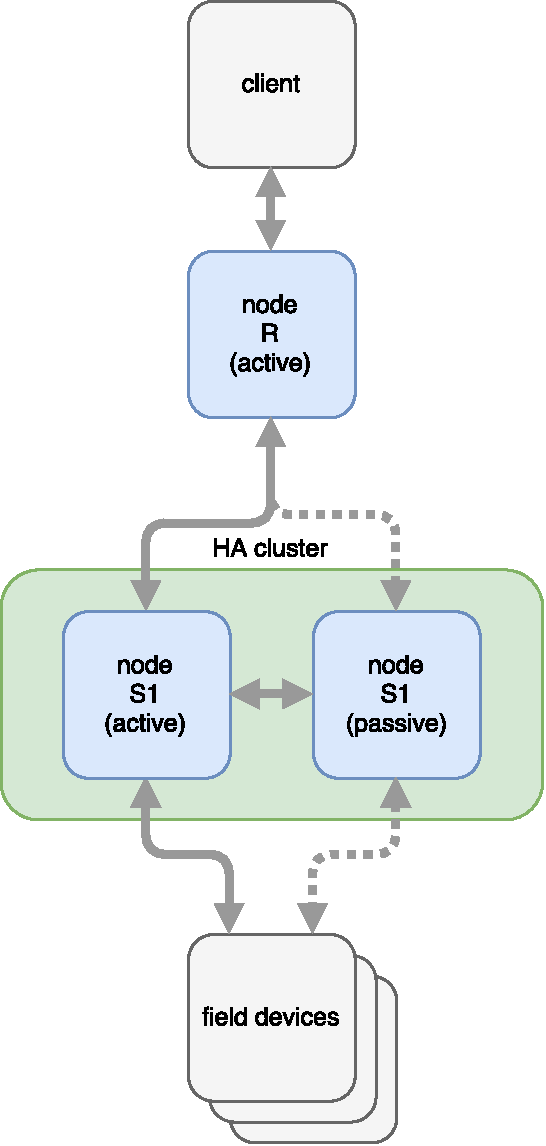
\includegraphics[width=0.5\textwidth]{img/ml_ha_on_sub_exotic_topology.pdf}
	\caption{Unusual federation example: Multi level, \gls{HA} at bottom}
	\label{fig:topo:exotic:ml:ha:on:sub}
\end{figure}

\begin{figure}[]
	\center
	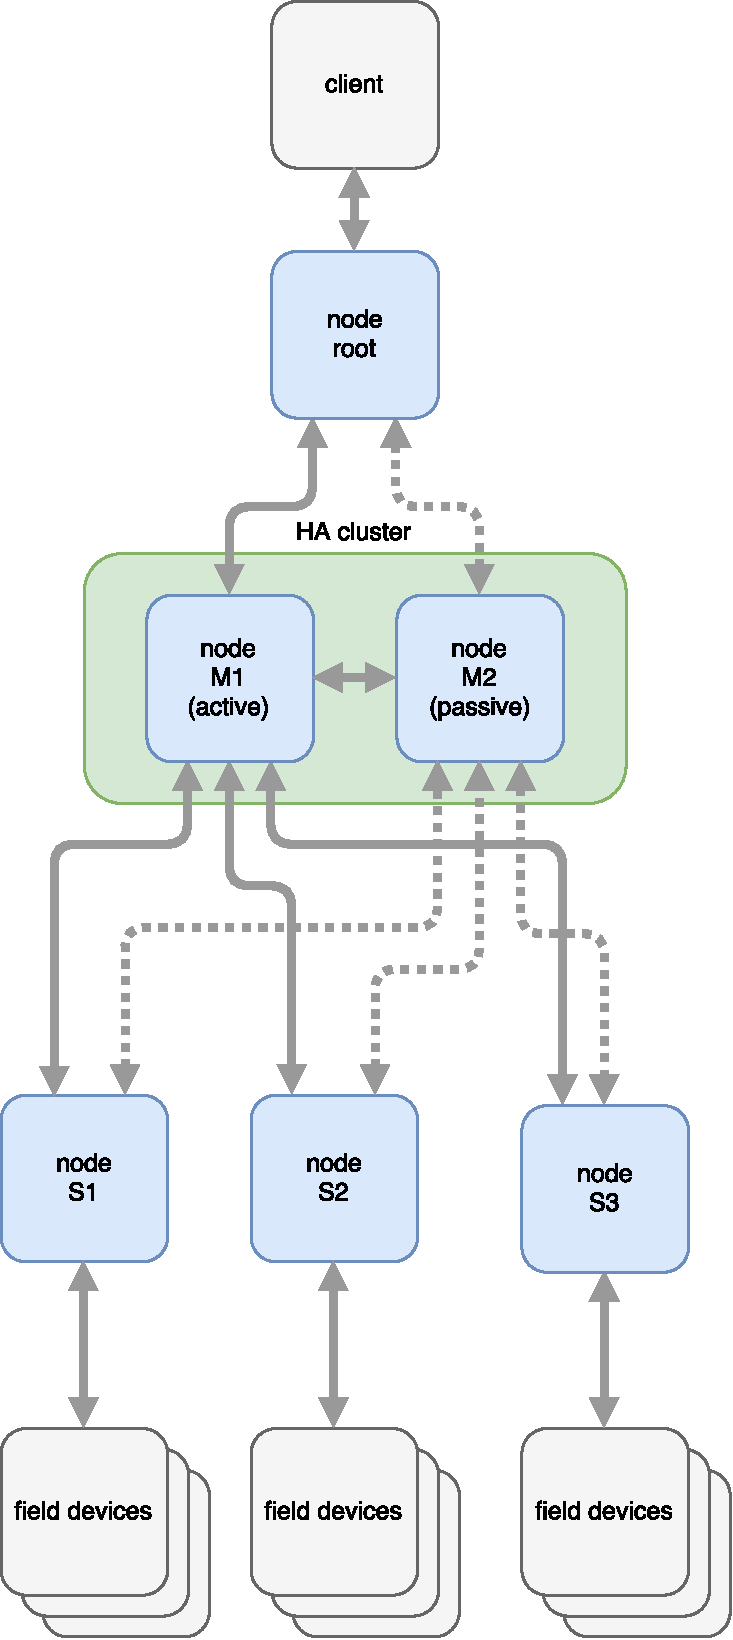
\includegraphics[width=0.5\textwidth]{img/ml_ha_on_mid_exotic_topology.pdf}
	\caption{Unusual Federation example: Multi level, \gls{HA} in the middle}
	\label{fig:topo:exotic:ml:ha:on:mid}
\end{figure}


\paragraph{Dedicated network link}
It is possible that there will be a dedicated, direct network link from one peer to
the other. However, this will not be the typical case.

\paragraph{Split-brain syndrome}
At initialization, the two peers must be able to automatically decide on which peer
becomes active first.  At any time, only one of the two HA peers must be
active (i.e. serving clients), and the other one must stay passive (i.e. ignore
client requests and only keep its DIM up-to-date). The passive HA peer shall
take over in the event that the currently active peer becomes unavailable.
Measures must be taken to avoid the dreaded split-brain syndrome where both HA
peers become active.

The types of failures that need to be handled include:
\begin{itemize}
	\item Software failure on the primary node, like an application or OS crash
	\item Hardware failure on the primary node, like a defect power supply
	\item Failure of a network link, completely disconnecting a HA peer from the federation
\end{itemize}

All three failure types listed can collectively be called \emph{crash},
as their effects are the same from the point of view of the whole federation.

The high availability requirement is formally specified in \autoref{lst:feature:ha}

\begin{listing}
	\inputminted{Gherkin}{listings/features/high_availability.feature}
	\caption{Formal feature: High availability}
	\label{lst:feature:ha}
\end{listing}

\section{Persistence replication}
% TODO: explain what south/north means, maybe in scope already
This is about the replication of persisted data, which is currently stored
in \gls{tc} databases on a Roadster node, one for each kind of data. With the federation functionality, this is
still true: Every node will have its own set of key-value stores. Changes to the persisted
data must flow from south to north (towards the root node), so the root
node can collect and maintain a replication of the persisted data of all
nodes within the federation, recursively.

Again, it is important that every node and its subnodes form an autonomous subsystem. So
in case the link to its supernode fails, it has to continue working. As soon as
the link is repaired, replication of the delta (changes to the data) can
be initiated.

This is different from \gls{DIM} replication, as the DIM is shared across
all nodes and is a relatively small data structure holding merely the current state. The \gls{tc} databases
can possibly contain large amounts of data (in the hundreds of megabytes) and
are shared only towards the root node (thus "bubbling up").

This is formally specified in \autoref{lst:feature:persistence_synchronization}.

\begin{listing}
	\inputminted{Gherkin}{listings/features/persistence_synchronization.feature}
	\caption{Formal feature: Persistence replication}
	\label{lst:feature:persistence_synchronization}
\end{listing}

% ---------------------------------------------------------------------------
\section{Non-functional requirements}\label{sec:nfr}
The following subsections elaborate on the non-functional requirements.

\subsection{Simplicity}
The two reoccuring patterns that surfaced during the requirements gathering
meeting were:

\begin{enumerate}
\item \gls{KISS} principle. Simplicity is favored, as experience shows that
	simpler systems are more stable, so complexity should be avoided if not
	absolutely necessary.

\item No premature optimization since it is the root of all evil.\footnote{Quote
	by Donald Knuth: ``Premature optimization is the root of all evil.''}
\end{enumerate}
% TODO: recycle ZMQ sockets


\subsection{Testing}
Regarding testing, the following requirements exist:
\begin{itemize}
	\item the student's contributions are verified using unit tests
	\item the formally described scenarios shall be verified using
		integration tests in a close-to-reality setup, either
		automatically or manually
\end{itemize}

\subsection{Constraints for persistence replication}
100\% consistency is not an absolute requirement for persistence replication.
Nor is zero data loss an absolut requirement. However, it is mandatory that
updates make it to the root node within 30 seconds.

\subsection{High availability for OPC UA}
The high availability feature shall be designed with \gls{opc-ua} in mind. It
should be easy to adapt it to the various kinds of server redundancies specified
in OPC-UA, including the transparent and non-transparent variants.

\subsection{Encryption}
\emph{This is optional. Also, this requirement has the lowest priority not
because it is insignificant, but because it is trivial to enable transport level
security on \zmq sockets later on.}

The inter-node communication of a Roadster federation must be secured using
encryption. Recent versions of \zmq offer modern, authenticated encryption,
including server and client authentication (the latter is optional).
The client favors a solution where every communication partner (a node)
authenticates all its communication partners, and vice versa.

Since the \zmq binding used in the legacy version is unmaintained and does not
allow encryption, it has to be exchanged with a more appropriate library.

\subsection{Code style}
The coding guidelines desired by the client are basically the ones written down
in the popular Ruby style guide \cite{rb:style-guide}, with the following
differences or special remarks:

\begin{itemize}
	\item Non-interpolated strings shall be written as \rb{'foobar'}, not \rb{"foobar"}.

	\item Method invocation: Parenthesis shall be omitted when unnecessary, even with
		arguments present. This is opposed to the rule
		\cite[\href{https://github.com/bbatsov/ruby-style-guide\#method-invocation-parens}{Method~Invocation~Syntax}]{rb:style-guide}.

	\item Method definitions shall be preceded by two blank lines. This slightly
		extends the rule
		\cite[\href{https://github.com/bbatsov/ruby-style-guide\#empty-lines-between-methods}{Source~Code~Layout}]{rb:style-guide}.

	\item Before and after API documentation there shall be one blank comment line for better readability. This ignores
		the rule \cite[\href{https://github.com/bbatsov/ruby-style-guide\#rdoc-conventions}{Source~Code~Layout}]{rb:style-guide}.

	\item Syntax sugar for Hashes with Symbol keys ($\geqslant$ Ruby 1.9)
		is required, as per rule
		\cite[\href{https://github.com/bbatsov/ruby-style-guide\#hash-literals}{Collections}]{rb:style-guide}.\\
		Example: \mintinline[bgcolor=bg]{Ruby};{ foo: "bar", baz: 42 }; instead of \mintinline[bgcolor=bg]{Ruby};{ :foo => "bar", :baz => 42 };

	\item Align multiple assignments so there is a column of equal signs.
\end{itemize}
